\documentclass{standalone}
\usepackage{tikz}
\usepackage{ctex,siunitx}
\setCJKmainfont{Noto Serif CJK SC}
\usepackage{tkz-euclide}
\usepackage{amsmath}
\usetikzlibrary{patterns, calc}
\usetikzlibrary {decorations.pathmorphing, decorations.pathreplacing, decorations.shapes,}
\begin{document}
\small
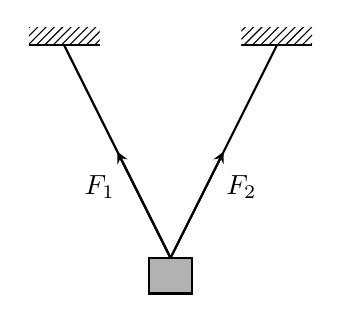
\begin{tikzpicture}[>=stealth, thick,scale=0.9]
  % \useasboundingbox(-1,-0.75)rectangle(3.7,1.4);
  \fill [pattern = north east lines] (-2,0) rectangle (-1,.25);
  \fill [pattern = north east lines] (1,0) rectangle (2,.25);
  \draw(-2,0)--(-1,0);  \draw(2,0)--(1,0);
  \draw (-1.5,0)--(0,-3);  \draw(1.5,0)--(0,-3);
  \draw[->] (0,-3)--(-.75,-1.5);  \draw[->] (0,-3)--(0.75,-1.5);
  \draw [fill=black!30] (-.3,-3.5) rectangle (.3,-3);
  \node at (-1,-2){$F_1$};\node at (1,-2){$F_2$};
  \end{tikzpicture}
\end{document}